\documentclass{article}

%%%%%%%%%%%%%%%%%%%%%%%%%%%%%%%%%
% PACKAGE IMPORTS
%%%%%%%%%%%%%%%%%%%%%%%%%%%%%%%%%


\usepackage[tmargin=2cm,rmargin=1in,lmargin=1in,margin=0.85in,bmargin=2cm,footskip=.2in]{geometry}
\usepackage{amsmath,amsfonts,amsthm,amssymb,mathtools}
% \usepackage[varbb]{newpxmath}
\usepackage{xfrac}
\usepackage[makeroom]{cancel}
\usepackage{mathtools}
\usepackage{bookmark}
\usepackage{enumitem}
\usepackage{hyperref,theoremref}
\hypersetup{
	pdftitle={Assignment},
	colorlinks=true, linkcolor=doc!90,
	bookmarksnumbered=true,
	bookmarksopen=true
}
\usepackage[most,many,breakable]{tcolorbox}
\usepackage{cancel}
\renewcommand{\CancelColor}{\color{red}} % bring in cancel & make it red...
\usepackage{xcolor}
\usepackage{varwidth}
\usepackage{varwidth}
\usepackage{etoolbox}
%\usepackage{authblk}
\usepackage{nameref}
\usepackage{multicol,array}
\usepackage{tikz-cd}
\usepackage[ruled,vlined,linesnumbered]{algorithm2e}
\usepackage{comment} % enables the use of multi-line comments (\ifx \fi) 
\usepackage{import}
\usepackage{xifthen}
\usepackage{pdfpages}
\usepackage{transparent}
\usepackage{pgfplots}
\usepackage{float}

\newcommand\mycommfont[1]{\footnotesize\ttfamily\textcolor{blue}{#1}}
\SetCommentSty{mycommfont}
\newcommand{\incfig}[1]{%
    \def\svgwidth{\columnwidth}
    \import{./figures/}{#1.pdf_tex}
}

\usepackage{tikzsymbols}
\renewcommand\qedsymbol{$\Laughey$}


%\usepackage{import}
%\usepackage{xifthen}
%\usepackage{pdfpages}
%\usepackage{transparent}


%%%%%%%%%%%%%%%%%%%%%%%%%%%%%%
% SELF MADE COLORS
%%%%%%%%%%%%%%%%%%%%%%%%%%%%%%



\definecolor{myg}{RGB}{56, 140, 70}
\definecolor{myb}{RGB}{45, 111, 177}
\definecolor{myr}{RGB}{199, 68, 64}
\definecolor{mytheorembg}{HTML}{F2F2F9}
\definecolor{mytheoremfr}{HTML}{00007B}
\definecolor{mylenmabg}{HTML}{FFFAF8}
\definecolor{mylenmafr}{HTML}{983b0f}
\definecolor{mypropbg}{HTML}{f2fbfc}
\definecolor{mypropfr}{HTML}{191971}
\definecolor{myexamplebg}{HTML}{F2FBF8}
\definecolor{myexamplefr}{HTML}{88D6D1}
\definecolor{myexampleti}{HTML}{2A7F7F}
\definecolor{mydefinitbg}{HTML}{E5E5FF}
\definecolor{mydefinitfr}{HTML}{3F3FA3}
\definecolor{notesgreen}{RGB}{0,162,0}
\definecolor{myp}{RGB}{197, 92, 212}
\definecolor{mygr}{HTML}{2C3338}
\definecolor{myred}{RGB}{127,0,0}
\definecolor{myyellow}{RGB}{169,121,69}
\definecolor{myexercisebg}{HTML}{F2FBF8}
\definecolor{myexercisefg}{HTML}{88D6D1}


%%%%%%%%%%%%%%%%%%%%%%%%%%%%
% TCOLORBOX SETUPS
%%%%%%%%%%%%%%%%%%%%%%%%%%%%

\setlength{\parindent}{1cm}
%================================
% THEOREM BOX
%================================

\tcbuselibrary{theorems,skins,hooks}
\newtcbtheorem[number within=section]{Theorem}{Theorem}
{%
	enhanced,
	breakable,
	colback = mytheorembg,
	frame hidden,
	boxrule = 0sp,
	borderline west = {2pt}{0pt}{mytheoremfr},
	sharp corners,
	detach title,
	before upper = \tcbtitle\par\smallskip,
	coltitle = mytheoremfr,
	fonttitle = \bfseries\sffamily,
	description font = \mdseries,
	separator sign none,
	segmentation style={solid, mytheoremfr},
}
{th}

\tcbuselibrary{theorems,skins,hooks}
\newtcbtheorem[number within=section]{theorem}{Theorem}
{%
	enhanced,
	breakable,
	colback = mytheorembg,
	frame hidden,
	boxrule = 0sp,
	borderline west = {2pt}{0pt}{mytheoremfr},
	sharp corners,
	detach title,
	before upper = \tcbtitle\par\smallskip,
	coltitle = mytheoremfr,
	fonttitle = \bfseries\sffamily,
	description font = \mdseries,
	separator sign none,
	segmentation style={solid, mytheoremfr},
}
{th}


\tcbuselibrary{theorems,skins,hooks}
\newtcolorbox{Theoremcon}
{%
	enhanced
	,breakable
	,colback = mytheorembg
	,frame hidden
	,boxrule = 0sp
	,borderline west = {2pt}{0pt}{mytheoremfr}
	,sharp corners
	,description font = \mdseries
	,separator sign none
}

%================================
% Corollery
%================================
\tcbuselibrary{theorems,skins,hooks}
\newtcbtheorem[number within=section]{Corollary}{Corollary}
{%
	enhanced
	,breakable
	,colback = myp!10
	,frame hidden
	,boxrule = 0sp
	,borderline west = {2pt}{0pt}{myp!85!black}
	,sharp corners
	,detach title
	,before upper = \tcbtitle\par\smallskip
	,coltitle = myp!85!black
	,fonttitle = \bfseries\sffamily
	,description font = \mdseries
	,separator sign none
	,segmentation style={solid, myp!85!black}
}
{th}
\tcbuselibrary{theorems,skins,hooks}
\newtcbtheorem[number within=section]{corollary}{Corollary}
{%
	enhanced
	,breakable
	,colback = myp!10
	,frame hidden
	,boxrule = 0sp
	,borderline west = {2pt}{0pt}{myp!85!black}
	,sharp corners
	,detach title
	,before upper = \tcbtitle\par\smallskip
	,coltitle = myp!85!black
	,fonttitle = \bfseries\sffamily
	,description font = \mdseries
	,separator sign none
	,segmentation style={solid, myp!85!black}
}
{th}


%================================
% LENMA
%================================

\tcbuselibrary{theorems,skins,hooks}
\newtcbtheorem[number within=section]{Lenma}{Lenma}
{%
	enhanced,
	breakable,
	colback = mylenmabg,
	frame hidden,
	boxrule = 0sp,
	borderline west = {2pt}{0pt}{mylenmafr},
	sharp corners,
	detach title,
	before upper = \tcbtitle\par\smallskip,
	coltitle = mylenmafr,
	fonttitle = \bfseries\sffamily,
	description font = \mdseries,
	separator sign none,
	segmentation style={solid, mylenmafr},
}
{th}

\tcbuselibrary{theorems,skins,hooks}
\newtcbtheorem[number within=section]{lenma}{Lenma}
{%
	enhanced,
	breakable,
	colback = mylenmabg,
	frame hidden,
	boxrule = 0sp,
	borderline west = {2pt}{0pt}{mylenmafr},
	sharp corners,
	detach title,
	before upper = \tcbtitle\par\smallskip,
	coltitle = mylenmafr,
	fonttitle = \bfseries\sffamily,
	description font = \mdseries,
	separator sign none,
	segmentation style={solid, mylenmafr},
}
{th}


%================================
% PROPOSITION
%================================

\tcbuselibrary{theorems,skins,hooks}
\newtcbtheorem[number within=section]{Prop}{Proposition}
{%
	enhanced,
	breakable,
	colback = mypropbg,
	frame hidden,
	boxrule = 0sp,
	borderline west = {2pt}{0pt}{mypropfr},
	sharp corners,
	detach title,
	before upper = \tcbtitle\par\smallskip,
	coltitle = mypropfr,
	fonttitle = \bfseries\sffamily,
	description font = \mdseries,
	separator sign none,
	segmentation style={solid, mypropfr},
}
{th}

\tcbuselibrary{theorems,skins,hooks}
\newtcbtheorem[number within=section]{prop}{Proposition}
{%
	enhanced,
	breakable,
	colback = mypropbg,
	frame hidden,
	boxrule = 0sp,
	borderline west = {2pt}{0pt}{mypropfr},
	sharp corners,
	detach title,
	before upper = \tcbtitle\par\smallskip,
	coltitle = mypropfr,
	fonttitle = \bfseries\sffamily,
	description font = \mdseries,
	separator sign none,
	segmentation style={solid, mypropfr},
}
{th}


%================================
% CLAIM
%================================

\tcbuselibrary{theorems,skins,hooks}
\newtcbtheorem[number within=section]{claim}{Claim}
{%
	enhanced
	,breakable
	,colback = myg!10
	,frame hidden
	,boxrule = 0sp
	,borderline west = {2pt}{0pt}{myg}
	,sharp corners
	,detach title
	,before upper = \tcbtitle\par\smallskip
	,coltitle = myg!85!black
	,fonttitle = \bfseries\sffamily
	,description font = \mdseries
	,separator sign none
	,segmentation style={solid, myg!85!black}
}
{th}



%================================
% Exercise
%================================

\tcbuselibrary{theorems,skins,hooks}
\newtcbtheorem[number within=section]{Exercise}{Exercise}
{%
	enhanced,
	breakable,
	colback = myexercisebg,
	frame hidden,
	boxrule = 0sp,
	borderline west = {2pt}{0pt}{myexercisefg},
	sharp corners,
	detach title,
	before upper = \tcbtitle\par\smallskip,
	coltitle = myexercisefg,
	fonttitle = \bfseries\sffamily,
	description font = \mdseries,
	separator sign none,
	segmentation style={solid, myexercisefg},
}
{th}

\tcbuselibrary{theorems,skins,hooks}
\newtcbtheorem[number within=section]{exercise}{Exercise}
{%
	enhanced,
	breakable,
	colback = myexercisebg,
	frame hidden,
	boxrule = 0sp,
	borderline west = {2pt}{0pt}{myexercisefg},
	sharp corners,
	detach title,
	before upper = \tcbtitle\par\smallskip,
	coltitle = myexercisefg,
	fonttitle = \bfseries\sffamily,
	description font = \mdseries,
	separator sign none,
	segmentation style={solid, myexercisefg},
}
{th}

%================================
% EXAMPLE BOX
%================================

\newtcbtheorem[number within=section]{Example}{Example}
{%
	colback = myexamplebg
	,breakable
	,colframe = myexamplefr
	,coltitle = myexampleti
	,boxrule = 1pt
	,sharp corners
	,detach title
	,before upper=\tcbtitle\par\smallskip
	,fonttitle = \bfseries
	,description font = \mdseries
	,separator sign none
	,description delimiters parenthesis
}
{ex}

\newtcbtheorem[number within=section]{example}{Example}
{%
	colback = myexamplebg
	,breakable
	,colframe = myexamplefr
	,coltitle = myexampleti
	,boxrule = 1pt
	,sharp corners
	,detach title
	,before upper=\tcbtitle\par\smallskip
	,fonttitle = \bfseries
	,description font = \mdseries
	,separator sign none
	,description delimiters parenthesis
}
{ex}

%================================
% DEFINITION BOX
%================================

\newtcbtheorem[number within=section]{Definition}{Definition}{enhanced,
	before skip=2mm,after skip=2mm, colback=red!5,colframe=red!80!black,boxrule=0.5mm,
	attach boxed title to top left={xshift=1cm,yshift*=1mm-\tcboxedtitleheight}, varwidth boxed title*=-3cm,
	boxed title style={frame code={
					\path[fill=tcbcolback]
					([yshift=-1mm,xshift=-1mm]frame.north west)
					arc[start angle=0,end angle=180,radius=1mm]
					([yshift=-1mm,xshift=1mm]frame.north east)
					arc[start angle=180,end angle=0,radius=1mm];
					\path[left color=tcbcolback!60!black,right color=tcbcolback!60!black,
						middle color=tcbcolback!80!black]
					([xshift=-2mm]frame.north west) -- ([xshift=2mm]frame.north east)
					[rounded corners=1mm]-- ([xshift=1mm,yshift=-1mm]frame.north east)
					-- (frame.south east) -- (frame.south west)
					-- ([xshift=-1mm,yshift=-1mm]frame.north west)
					[sharp corners]-- cycle;
				},interior engine=empty,
		},
	fonttitle=\bfseries,
	title={#2},#1}{def}
\newtcbtheorem[number within=section]{definition}{Definition}{enhanced,
	before skip=2mm,after skip=2mm, colback=red!5,colframe=red!80!black,boxrule=0.5mm,
	attach boxed title to top left={xshift=1cm,yshift*=1mm-\tcboxedtitleheight}, varwidth boxed title*=-3cm,
	boxed title style={frame code={
					\path[fill=tcbcolback]
					([yshift=-1mm,xshift=-1mm]frame.north west)
					arc[start angle=0,end angle=180,radius=1mm]
					([yshift=-1mm,xshift=1mm]frame.north east)
					arc[start angle=180,end angle=0,radius=1mm];
					\path[left color=tcbcolback!60!black,right color=tcbcolback!60!black,
						middle color=tcbcolback!80!black]
					([xshift=-2mm]frame.north west) -- ([xshift=2mm]frame.north east)
					[rounded corners=1mm]-- ([xshift=1mm,yshift=-1mm]frame.north east)
					-- (frame.south east) -- (frame.south west)
					-- ([xshift=-1mm,yshift=-1mm]frame.north west)
					[sharp corners]-- cycle;
				},interior engine=empty,
		},
	fonttitle=\bfseries,
	title={#2},#1}{def}



%================================
% Solution BOX
%================================

\makeatletter
\newtcbtheorem{question}{Question}{enhanced,
	breakable,
	colback=white,
	colframe=myb!80!black,
	attach boxed title to top left={yshift*=-\tcboxedtitleheight},
	fonttitle=\bfseries,
	title={#2},
	boxed title size=title,
	boxed title style={%
			sharp corners,
			rounded corners=northwest,
			colback=tcbcolframe,
			boxrule=0pt,
		},
	underlay boxed title={%
			\path[fill=tcbcolframe] (title.south west)--(title.south east)
			to[out=0, in=180] ([xshift=5mm]title.east)--
			(title.center-|frame.east)
			[rounded corners=\kvtcb@arc] |-
			(frame.north) -| cycle;
		},
	#1
}{def}
\makeatother

%================================
% SOLUTION BOX
%================================

\makeatletter
\newtcolorbox{solution}{enhanced,
	breakable,
	colback=white,
	colframe=myg!80!black,
	attach boxed title to top left={yshift*=-\tcboxedtitleheight},
	title=Solution,
	boxed title size=title,
	boxed title style={%
			sharp corners,
			rounded corners=northwest,
			colback=tcbcolframe,
			boxrule=0pt,
		},
	underlay boxed title={%
			\path[fill=tcbcolframe] (title.south west)--(title.south east)
			to[out=0, in=180] ([xshift=5mm]title.east)--
			(title.center-|frame.east)
			[rounded corners=\kvtcb@arc] |-
			(frame.north) -| cycle;
		},
}
\makeatother

%================================
% Question BOX
%================================

\makeatletter
\newtcbtheorem{qstion}{Question}{enhanced,
	breakable,
	colback=white,
	colframe=mygr,
	attach boxed title to top left={yshift*=-\tcboxedtitleheight},
	fonttitle=\bfseries,
	title={#2},
	boxed title size=title,
	boxed title style={%
			sharp corners,
			rounded corners=northwest,
			colback=tcbcolframe,
			boxrule=0pt,
		},
	underlay boxed title={%
			\path[fill=tcbcolframe] (title.south west)--(title.south east)
			to[out=0, in=180] ([xshift=5mm]title.east)--
			(title.center-|frame.east)
			[rounded corners=\kvtcb@arc] |-
			(frame.north) -| cycle;
		},
	#1
}{def}
\makeatother

\newtcbtheorem[number within=section]{wconc}{Wrong Concept}{
	breakable,
	enhanced,
	colback=white,
	colframe=myr,
	arc=0pt,
	outer arc=0pt,
	fonttitle=\bfseries\sffamily\large,
	colbacktitle=myr,
	attach boxed title to top left={},
	boxed title style={
			enhanced,
			skin=enhancedfirst jigsaw,
			arc=3pt,
			bottom=0pt,
			interior style={fill=myr}
		},
	#1
}{def}



%================================
% NOTE BOX
%================================

\usetikzlibrary{arrows,calc,shadows.blur}
\tcbuselibrary{skins}
\newtcolorbox{note}[1][]{%
	enhanced jigsaw,
	colback=gray!20!white,%
	colframe=gray!80!black,
	size=small,
	boxrule=1pt,
	title=\textbf{Note:-},
	halign title=flush center,
	coltitle=black,
	breakable,
	drop shadow=black!50!white,
	attach boxed title to top left={xshift=1cm,yshift=-\tcboxedtitleheight/2,yshifttext=-\tcboxedtitleheight/2},
	minipage boxed title=1.5cm,
	boxed title style={%
			colback=white,
			size=fbox,
			boxrule=1pt,
			boxsep=2pt,
			underlay={%
					\coordinate (dotA) at ($(interior.west) + (-0.5pt,0)$);
					\coordinate (dotB) at ($(interior.east) + (0.5pt,0)$);
					\begin{scope}
						\clip (interior.north west) rectangle ([xshift=3ex]interior.east);
						\filldraw [white, blur shadow={shadow opacity=60, shadow yshift=-.75ex}, rounded corners=2pt] (interior.north west) rectangle (interior.south east);
					\end{scope}
					\begin{scope}[gray!80!black]
						\fill (dotA) circle (2pt);
						\fill (dotB) circle (2pt);
					\end{scope}
				},
		},
	#1,
}

%%%%%%%%%%%%%%%%%%%%%%%%%%%%%%
% SELF MADE COMMANDS
%%%%%%%%%%%%%%%%%%%%%%%%%%%%%%


\newcommand{\thm}[2]{\begin{Theorem}{#1}{}#2\end{Theorem}}
\newcommand{\cor}[2]{\begin{Corollary}{#1}{}#2\end{Corollary}}
\newcommand{\mlenma}[2]{\begin{Lenma}{#1}{}#2\end{Lenma}}
\newcommand{\mprop}[2]{\begin{Prop}{#1}{}#2\end{Prop}}
\newcommand{\clm}[3]{\begin{claim}{#1}{#2}#3\end{claim}}
\newcommand{\wc}[2]{\begin{wconc}{#1}{}\setlength{\parindent}{1cm}#2\end{wconc}}
\newcommand{\thmcon}[1]{\begin{Theoremcon}{#1}\end{Theoremcon}}
\newcommand{\ex}[2]{\begin{Example}{#1}{}#2\end{Example}}
\newcommand{\dfn}[2]{\begin{Definition}[colbacktitle=red!75!black]{#1}{}#2\end{Definition}}
\newcommand{\dfnc}[2]{\begin{definition}[colbacktitle=red!75!black]{#1}{}#2\end{definition}}
\newcommand{\qs}[2]{\begin{question}{#1}{}#2\end{question}}
\newcommand{\pf}[2]{\begin{myproof}[#1]#2\end{myproof}}
\newcommand{\nt}[1]{\begin{note}#1\end{note}}

\newcommand*\circled[1]{\tikz[baseline=(char.base)]{
		\node[shape=circle,draw,inner sep=1pt] (char) {#1};}}
\newcommand\getcurrentref[1]{%
	\ifnumequal{\value{#1}}{0}
	{??}
	{\the\value{#1}}%
}
\newcommand{\getCurrentSectionNumber}{\getcurrentref{section}}
\newenvironment{myproof}[1][\proofname]{%
	\proof[\bfseries #1: ]%
}{\endproof}

\newcommand{\mclm}[2]{\begin{myclaim}[#1]#2\end{myclaim}}
\newenvironment{myclaim}[1][\claimname]{\proof[\bfseries #1: ]}{}

\newcounter{mylabelcounter}

\makeatletter
\newcommand{\setword}[2]{%
	\phantomsection
	#1\def\@currentlabel{\unexpanded{#1}}\label{#2}%
}
\makeatother




\tikzset{
	symbol/.style={
			draw=none,
			every to/.append style={
					edge node={node [sloped, allow upside down, auto=false]{$#1$}}}
		}
}


% deliminators
\DeclarePairedDelimiter{\abs}{\lvert}{\rvert}
\DeclarePairedDelimiter{\norm}{\lVert}{\rVert}

\DeclarePairedDelimiter{\ceil}{\lceil}{\rceil}
\DeclarePairedDelimiter{\floor}{\lfloor}{\rfloor}
\DeclarePairedDelimiter{\round}{\lfloor}{\rceil}

\newsavebox\diffdbox
\newcommand{\slantedromand}{{\mathpalette\makesl{d}}}
\newcommand{\makesl}[2]{%
\begingroup
\sbox{\diffdbox}{$\mathsurround=0pt#1\mathrm{#2}$}%
\pdfsave
\pdfsetmatrix{1 0 0.2 1}%
\rlap{\usebox{\diffdbox}}%
\pdfrestore
\hskip\wd\diffdbox
\endgroup
}
\newcommand{\dd}[1][]{\ensuremath{\mathop{}\!\ifstrempty{#1}{%
\slantedromand\@ifnextchar^{\hspace{0.2ex}}{\hspace{0.1ex}}}%
{\slantedromand\hspace{0.2ex}^{#1}}}}
\ProvideDocumentCommand\dv{o m g}{%
  \ensuremath{%
    \IfValueTF{#3}{%
      \IfNoValueTF{#1}{%
        \frac{\dd #2}{\dd #3}%
      }{%
        \frac{\dd^{#1} #2}{\dd #3^{#1}}%
      }%
    }{%
      \IfNoValueTF{#1}{%
        \frac{\dd}{\dd #2}%
      }{%
        \frac{\dd^{#1}}{\dd #2^{#1}}%
      }%
    }%
  }%
}
\providecommand*{\pdv}[3][]{\frac{\partial^{#1}#2}{\partial#3^{#1}}}
%  - others
\DeclareMathOperator{\Lap}{\mathcal{L}}
\DeclareMathOperator{\Var}{Var} % varience
\DeclareMathOperator{\Cov}{Cov} % covarience
\DeclareMathOperator{\E}{E} % expected

% Since the amsthm package isn't loaded

% I prefer the slanted \leq
\let\oldleq\leq % save them in case they're every wanted
\let\oldgeq\geq
\renewcommand{\leq}{\leqslant}
\renewcommand{\geq}{\geqslant}

% % redefine matrix env to allow for alignment, use r as default
% \renewcommand*\env@matrix[1][r]{\hskip -\arraycolsep
%     \let\@ifnextchar\new@ifnextchar
%     \array{*\c@MaxMatrixCols #1}}


%\usepackage{framed}
%\usepackage{titletoc}
%\usepackage{etoolbox}
%\usepackage{lmodern}


%\patchcmd{\tableofcontents}{\contentsname}{\sffamily\contentsname}{}{}

%\renewenvironment{leftbar}
%{\def\FrameCommand{\hspace{6em}%
%		{\color{myyellow}\vrule width 2pt depth 6pt}\hspace{1em}}%
%	\MakeFramed{\parshape 1 0cm \dimexpr\textwidth-6em\relax\FrameRestore}\vskip2pt%
%}
%{\endMakeFramed}

%\titlecontents{chapter}
%[0em]{\vspace*{2\baselineskip}}
%{\parbox{4.5em}{%
%		\hfill\Huge\sffamily\bfseries\color{myred}\thecontentspage}%
%	\vspace*{-2.3\baselineskip}\leftbar\textsc{\small\chaptername~\thecontentslabel}\\\sffamily}
%{}{\endleftbar}
%\titlecontents{section}
%[8.4em]
%{\sffamily\contentslabel{3em}}{}{}
%{\hspace{0.5em}\nobreak\itshape\color{myred}\contentspage}
%\titlecontents{subsection}
%[8.4em]
%{\sffamily\contentslabel{3em}}{}{}  
%{\hspace{0.5em}\nobreak\itshape\color{myred}\contentspage}



%%%%%%%%%%%%%%%%%%%%%%%%%%%%%%%%%%%%%%%%%%%
% TABLE OF CONTENTS
%%%%%%%%%%%%%%%%%%%%%%%%%%%%%%%%%%%%%%%%%%%

% \usepackage{tikz}
% \definecolor{doc}{RGB}{0,60,110}
% \usepackage{titletoc}
% \contentsmargin{0cm}
% % \titlecontents{chapter}[3.7pc]
% {\addvspace{30pt}%
% 	\begin{tikzpicture}[remember picture, overlay]%
% 		\draw[fill=doc!60,draw=doc!60] (-7,-.1) rectangle (-0.9,.5);%
% 		\pgftext[left,x=-3.5cm,y=0.2cm]{\color{white}\Large\sc\bfseries Section\ \thecontentslabel};%
% 	\end{tikzpicture}\color{doc!60}\large\sc\bfseries}%
% {}
% {}
% {\;\titlerule\;\large\sc\bfseries Page \thecontentspage
% 	\begin{tikzpicture}[remember picture, overlay]
% 		\draw[fill=doc!60,draw=doc!60] (2pt,0) rectangle (4,0.1pt);
% 	\end{tikzpicture}}%
% \titlecontents{section}[3.7pc]
% {\addvspace{2pt}}
% {\contentslabel[\thecontentslabel]{2pc}}
% {}
% {\hfill\small \thecontentspage}
% []
% \titlecontents*{subsection}[3.7pc]
% {\addvspace{-1pt}\small}
% {}
% {}
% {\ --- \small\thecontentspage}
% [ \textbullet\ ][]

% \makeatletter
% \renewcommand{\tableofcontents}{%
% 	% \chapter*{%
% 	  \vspace*{-20\p@}%
% 	  \begin{tikzpicture}[remember picture, overlay]%
% 		  \pgftext[right,x=15cm,y=0.2cm]{\color{doc!60}\Huge\sc\bfseries \contentsname};%
% 		  \draw[fill=doc!60,draw=doc!60] (13,-.75) rectangle (20,1);%
% 		  \clip (13,-.75) rectangle (20,1);
% 		  \pgftext[right,x=15cm,y=0.2cm]{\color{white}\Huge\sc\bfseries \contentsname};%
% 	  \end{tikzpicture}}%
% 	\@starttoc{toc}}
% \makeatother

\newcommand{\ub}[1]{\underbar{$#1$}}

\newcommand{\p}[3]{\left( \frac{\partial #1}{\partial #2} \right)_{#3}}

\newcommand{\pop}[2]{\left.\frac{\partial}{\partial #1} \right\vert_{#2}}

\newcommand{\highlight}[2]{\colorbox{#1!20}{$\displaystyle#2$}}

\newcommand{\centmini}[2]{%
	\begin{center}
		\begin{minipage}{#1\linewidth}
			#2
		\end{minipage}
	\end{center}
}

\usepackage{tikz-3dplot}
\usepackage{booktabs}
\usepackage{titling}
\usepackage{fancyhdr}
\usetikzlibrary{patterns}
\usepackage{pgfplots}
\pgfplotsset{compat=1.18}

\usepackage{tcolorbox}
\usepackage[export]{adjustbox}
\usepackage{tikz}

\tcbset{colback=blue!7!white}
\tcbsetforeverylayer{colframe=blue!75!black}


\pretitle{\vspace{-4em}\begin{flushleft}\LARGE} % Adjust the size and alignment
    \posttitle{\end{flushleft}}
    \preauthor{\begin{flushleft}\large} % Adjust the size and alignment
    \postauthor{\hspace{2em} \large \thedate\end{flushleft}} % Place author and date on the same line
    \predate{} % Remove the default date formatting
    \postdate{} % Remove the default date formatting

\pagestyle{fancy}
\fancyhf{} % Clear all header and footer fields
\fancyfoot[R]{\thepage} % Right-align the page number in the footer
\renewcommand{\headrulewidth}{0pt} % Remove the header rule
\renewcommand{\footrulewidth}{0pt} % Remove the footer rule
\setlength{\fboxrule}{1pt}

\geometry{
    top=1.2cm,    % Top margin
    bottom=3cm, % Bottom margin
    left=1.0cm, % Left margin
    right=1.0cm % Right margin
}
\title{\bfseries CHEG325 E1 Cheatsheets}
\author{Kyle Wodehouse}
\date{}

\begin{document}
\maketitle

\begin{minipage}[t]{0.5\textwidth}
     \subsection*{fundamental relations}
        pure components
        \[
        dU = TdS - PdV + \underline{G} dN
        \]
        \[
        dH = T dS + V dP + \underline{G} dN
        \]
        \[
        dA = -P dV - S dT + \underline{G} dN
        \]
        \[
        dG = V dP - S dT + \underline{G} dN
        \]
        mixtures 
        \[
        dU = T dS - P dV + \sum^C_{i=1} {\mu}_{i} dN_{i}
        \]
    \subsection*{partial def of variables}

    \begin{align*}
    \underline{G} &= \left(\frac{\partial U}{\partial N}\right)_{S,V} = \left(\frac{\partial H}{\partial N}\right)_{P,S} = \left(\frac{\partial A}{\partial N}\right)_{T,V} \\[6pt]
                 &= \left(\frac{\partial G}{\partial N}\right)_{T,P} = -T\left(\frac{\partial S}{\partial N}\right)_{U,V}
    \end{align*}
    \begin{align*}
    \bar{G}_{i}  &= \left(\frac{ \partial U }{ \partial N_{i} } \right)_{S,V,N_{j\neq i}}
                  = \left(\frac{ \partial A }{ \partial N_{i} } \right)_{T,V,N_{j \neq i}} \\
                 &= \left(\frac{ \partial H }{ \partial N_{i} } \right)_{S,P}
                  = \left(\frac{ \partial G }{ \partial N_{i} } \right)_{T,P,N_{j \neq i}}
    \end{align*}
    \[
    S =  -\left(\frac{ \partial G }{ \partial T } \right)_{P} = -\left(\frac{ \partial A }{ \partial T } \right)_{V} 
    \]
    \subsection*{ideal gas things}
    \[\underline{U}^{\text{IG}}  = C_v^* T\]
    \[\underline{H}^{\text{IG}}  = C_p^* T\]
    \[\Delta S^{\text{IG}} = C_p \ln \frac{T_2}{T_1} - R \ln \frac{P_2}{P_1}\]
    \[\Delta G^{\text{IG}} \biggl\lvert_T = RT \ln \frac{P_2}{P_1}\]
    \subsection*{legendre (wrt $\xi_1$)}
    \[\tilde{\theta} \equiv \theta - \left(\frac{ \partial \theta }{ \partial \xi_{1} } \right)_{\xi_{j \neq 1}} \xi_{1} = \theta - \tilde{\xi}_{1} \xi_{1}  \]
    \[\left(\frac{ \partial \tilde{\theta} }{ \partial \tilde{\xi}_{1} } \right)_{\xi_{2}, \xi_{3}\dots}  = - \xi_{1}\]
\end{minipage}
\begin{minipage}[t]{0.48\textwidth}
    \subsection*{volterra}
    \[\left(\frac{ \delta g }{ \delta x_{i} } \right) = \left(\frac{ \partial g }{ \partial x_{i} } \right)_{} - \frac{1}{C} \sum_{j=1}^{C} \left(\frac{ \partial g }{ \partial x_{j} } \right)_{}  \]
    \[\bar{g}_{i} = g + \left(\frac{ \partial g }{ \partial x_{i} } \right)_{} - \sum_{j=1}^C \left(\frac{ \partial g }{ \partial x_{j} } \right)_{} x_{j}   \]
    \subsection*{partial molar property} 
    \[ \bar{\theta}_i (T,P,\underline{x}) = \left( \frac{\partial ( N\underline\theta)}{\partial N_i} \right)_{T,P,} \]
    \[{ \Delta_{\text{mix}} \theta = \sum_{i=1}^{\mathcal{C}} N_i \left[ \bar V_i - \underline V_i \right] } = \theta - \sum_{i=1}^{\mathcal{C}} N_i \underline\theta_i \]
    \subsection*{gibbs-duhem}
    \[ \sum N_{i} d\bar{\theta}\,\bigl\lvert_{T,P} = 0  \]
    \[ \sum x_{i} d\bar{\theta}\,\bigl\lvert_{T,P} = 0 \]
    \[x_{1}\left(\frac{ \partial \bar{\theta}_{1} }{ \partial x_{1} } \right)_{T,P} +x_{2}\left(\frac{ \partial \bar{\theta}_{2} }{ \partial x_{1} } \right)_{T,P} = 0\]
    \subsection*{reactions}
    \[\alpha A + \beta B \longleftrightarrow \rho R + \dots\]
    - products positive, reactants negative, inerts 0
    \[X \equiv \frac{N_{i} - N_{i,0}}{\nu_{i}}\]
    \[N_{i} = N_{i,0} + \nu_{i}X\]
    \subsection*{independent reactions}
    \subsubsection*{given reactions, use \underline{\underline{k}}}
    - column for each component, row for each reaction
    \[\text{rank}(\mathbf{k}) = \text{number of independent reactions}\]
    \subsubsection*{given components, use \underline{\underline{a}}}
    - column for each component, row for elements
    \[S = \text{rank}(\mathbf{a})\]
    \[I = C - S\]
\end{minipage}
\pagebreak

\begin{minipage}[t]{0.5\textwidth}
    \subsubsection*{reacting systems}
    mass balance for reacting system
    \[\frac{dN}{dt} = \sum_{k}^K \dot{N}_{k} + \sum_{i} \sum_{j} \nu_{ij} \dot{X}_{j}\]
    energy balance for reacting system
    \[\frac{dU}{dt} = \sum_{k}^K(\dot{N}\underline{H})_{k} + \dot{Q} + W_{s} -P \frac{dV}{dt}\]
    for CSTR
    \[\frac{dU}{dt} = \sum^{C} (\dot{N}\underline{H})_{in} + \sum^{C} (\dot{N}\underline{H})_{out} + \dot{Q} \]
    \subsubsection*{standard state heats of reactions}
    \[\Delta_{\text{rxn}} H^{\circ} = \sum_{i} \nu_{i}\Delta_{\text{form}} \underline{H}_{i}^{\circ}\]
    \subsection*{pmp from experiment}
    \[\Delta_{\text{mix}} \underline{V} - x_{1} \left(\frac{ \partial \Delta \underline{V} }{ \partial x_{1} } \right)_{T,P} = (\bar{V}_{2} - \underline{V}_{2})\]
    \subsection*{gibbs phase rule}
    \[\mathcal{F} = C - M - P + 2\]
    \subsection*{partial pressure; fugacity}
    \[P_{i} = x_{i}P_{\text{total}}\]
    fugacity using ideal gas mixture as reference
    \begin{align*}
        \bar{f}(T,P,\underline{x}) &= P_i \exp \left( \frac{\bar{G}_{i} (T,P,\underline{x}) - \bar{G}_{i}^{\text{IGM}}(T,P,\underline{x})}{RT} \right)  \\ \\
        &= P_i \exp \left( \frac{1}{RT} \int_{0}^P (\bar{V}_{i}- \bar{V}_{i}^{\text{IG}})\,dP \right)
    \end{align*} 
    \begin{minipage}[t]{0.47\textwidth}
        ideal mixture
        \[\bar{f}_{i}^{\text{IM}} = x_{i}f_{i}(T,P)\]
    \end{minipage}
    \begin{minipage}[t]{0.47\textwidth}
        ideal gas mixture
        \[ \bar{f}_{i}^{\text{IGM}} = x_{i} P_{\text{total}} \]
    \end{minipage}
    
    

    from eos
    \begin{align*}
        \ln \bar{\phi}  &= \frac{1}{RT}\int_{\infty}^{ZRT/P} \biggl[  \frac{RT}{V} - N \left(\frac{ \partial P }{ \partial N_{i} } \right)_{T,V,N_{j \neq i}} \biggr] \, d\underline{V} - \ln Z \\
        &= \ln \frac{\bar{f}_i}{x_i P}
    \end{align*}
    fugacity coefficient
    \[ \bar{\phi_i} = \frac{\bar{f}_i}{x_i P}\]


\end{minipage}
\begin{minipage}[t]{0.47\textwidth}
    \begin{center}
        \begin{tabular}{@{}lll@{}}
            \toprule
            property                                  & ideal gas mixture                           & $\Delta_{\text{mix}}\theta$ \\ \midrule
            $\bar{U}^{\text{IGM}}$                    & $\underline{U}^{\text{IG}}$                    & 0                           \\
            $\bar{H}^{\text{IGM}}$                    & $\underline{H}^{\text{IG}}$                    & 0                           \\
            $\bar{V}^{\text{IGM}}$ & $\underline{V}^{\text{IG}}(T,P)$               & 0                           \\
            $\bar{S}^{\text{IGM}}$ & $\underline{S}^{\text{IG}}(T,P) - R \ln x_{i}$  & $-R \sum x_{i} \ln x_{i}$   \\
            $\bar{G}^{\text{IGM}}$                    & $\underline{G}^{\text{IG}}(T,P) + RT \ln x_{i}$ & $RT \sum x_{i} \ln x_{i}$   \\ 
            $\bar{A}^{\text{IGM}}$                    & $\underline{A}^{\text{IG}}(T,P) + RT \ln x_{i}$ & $RT \sum x_{i} \ln x_{i}$   \\ 
            \bottomrule
        \end{tabular}
        \begin{tabular}{@{}lll@{}}
            \toprule
            property                                  & ideal mixture                           & $\Delta_{\text{mix}}\theta$ \\ \midrule
            $\underline{U}^{\text{IM}}$                    & $\sum x_i \underline{U}_i$                    & 0                           \\
            $\underline{H}^{\text{IM}}$                    & $\sum x_i \underline{H}_i$                    & 0                           \\
            $\underline{V}^{\text{IM}}$                           & $\sum x_i \underline{V}$               & 0                           \\
            $\underline{S}^{\text{IM}}$                     & $\sum x_i \underline{S}_i - R \sum x_i \ln x_{i}$  & $-R \sum x_{i} \ln x_{i}$   \\
            $\underline{A}^{\text{IM}}$                     & $\sum x_i \underline{A}_i + RT \sum x_i \ln x_{i}$  & $RT \sum x_{i} \ln x_{i}$   \\
            $\underline{G}^{\text{IM}}$                     & $\sum x_i \underline{G}_i + RT \sum x_i \ln x_{i}$  & $RT \sum x_{i} \ln x_{i}$   \\
            $\bar{S}^{\text{IM}}_i$                     & $\underline{S}_i(T,P) - R \ln x_{i}$  & $-R \sum x_{i} \ln x_{i}$   \\
            $\bar{A}^{\text{IM}}_i$                    & $\underline{A}_i(T,P) + RT \ln x_{i}$ & $RT \sum x_{i} \ln x_{i}$   \\ 
            $\bar{G}^{\text{IM}}_i$                    & $\underline{G}_i(T,P) + RT \ln x_{i}$ & $RT \sum x_{i} \ln x_{i}$   \\             
            \bottomrule
        \end{tabular}
    \end{center}
    excess properties
    \[\bar{\theta}^{\text{ex}}_i = \bar{\theta}_{i} - \bar{\theta}^{\text{IM}}_{i}\]
    \[\Delta_{\text{mix}}\underline{\theta} (T,P,\underline{x}) = \Delta_{\text{mix}}\underline{\theta}^{\text{IM}}(T,P,\underline{x}) + \underline{\theta}^{\text{ex}}\]
    excess gibbs
    \begin{align*}
        \bar{G}^{\text{ex}}_{i} &= \left(\frac{ \partial N \underline{G}^{\text{ex}} }{ \partial N_{i} } \right)_{T,P,N_{j \neq i}}  
        = RT \ln \left( \frac{\bar{f}_{i}}{x_{i}f_{i}} \right)  \\ 
        &= RT \ln\left( \frac{\bar{\phi}_{i}}{\phi_{i}} \right) 
        = \int_{0}^P \bar{V}_{i} - \underline{V}_{i} \ dP
    \end{align*}
    activity coefficient
    \[\gamma_{i} = \frac{\bar{f}_{i}}{x_{i} f_{i}} = \frac{\bar{\phi}_{i}}{\phi_{i}} \]
    \[RT \ln (\gamma_{i}) = \bar{G}_{i}^{ex}\]
    g-d for activity coefficients
    \[\sum x_{i} d\ln \gamma_{i} = 0\]
    lewis randall rule (low or high pressure)
    \[\bar{f}_{i} = y_{i} f_{i} \]
    \subsection*{VLE}
    low pressure vle
    \[x_{i} \gamma_{i} P^{\text{vap}}_{i} = y_{i}P_{\text{total}}\]
    low pressure; ideal liquid; raoults
    \[x_{i} P^{\text{vap}}_{i} = y_{i} P_{\text{total}} \]
\end{minipage}

\begin{figure}[H]
    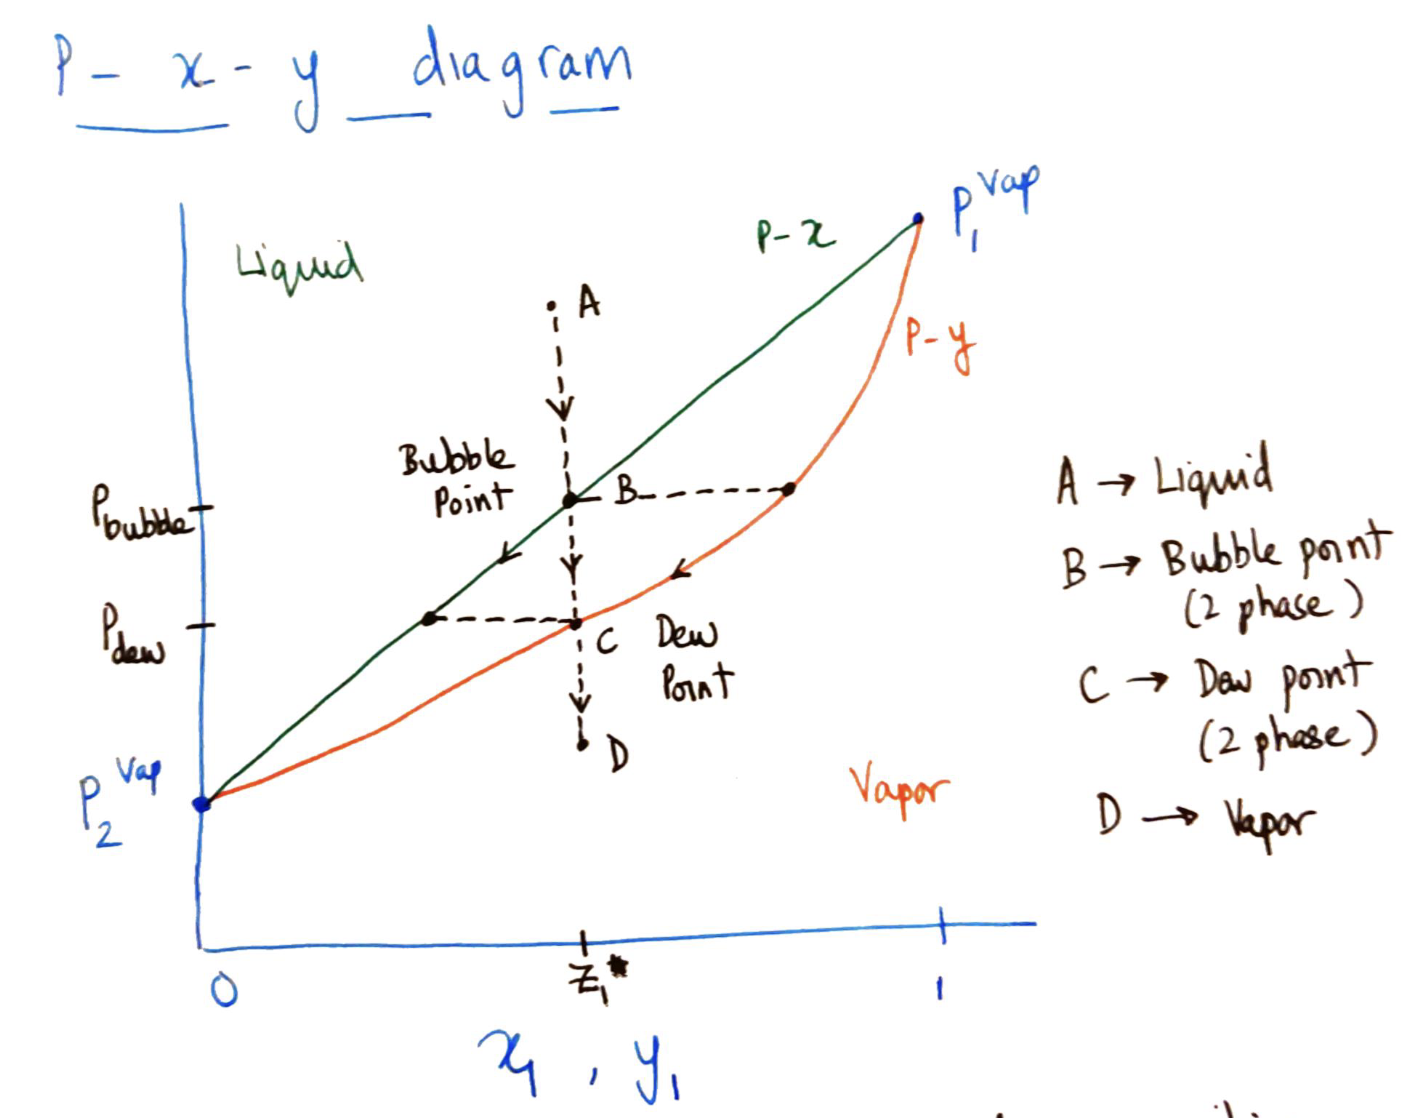
\includegraphics[width=0.52\textwidth, frame]{pxy.png}
    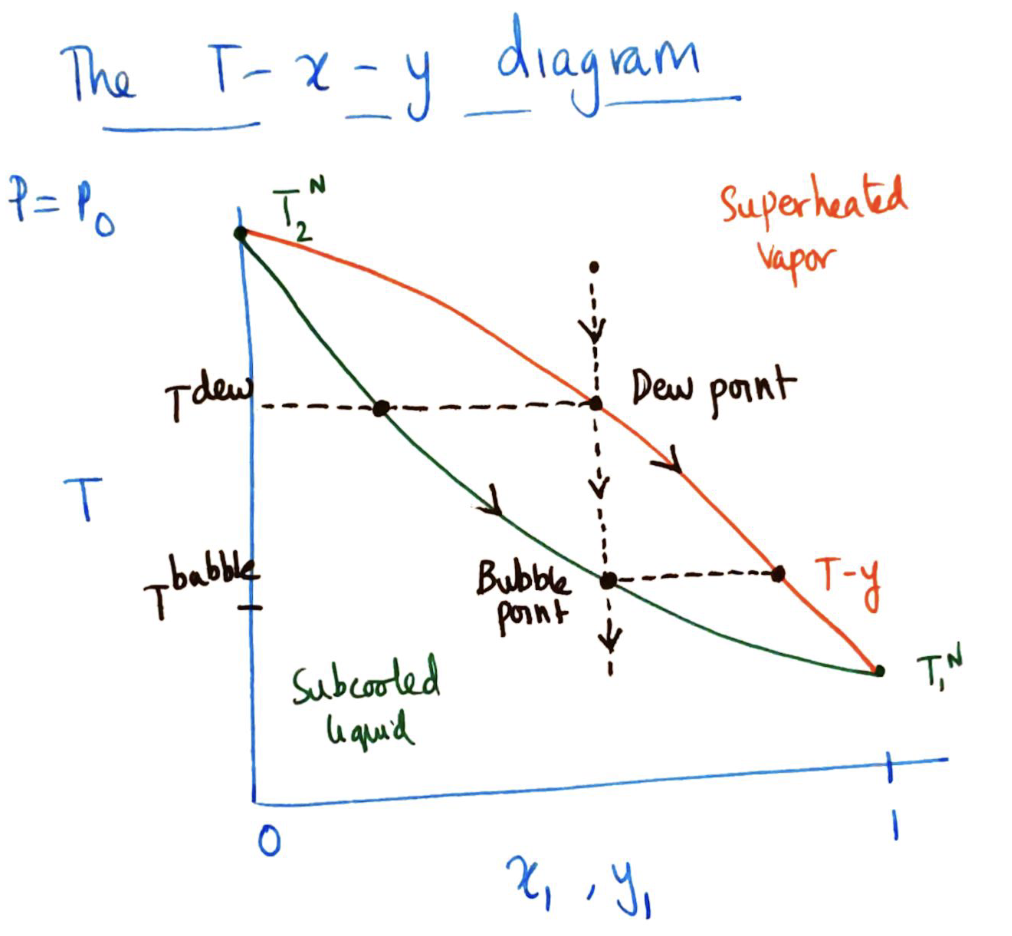
\includegraphics[width=0.442\textwidth, frame]{txy.png}
\end{figure}
\begin{minipage}[t]{0.47\textwidth}
    useful vle problem solutions
    \[\sum x_{i} P^{\text{vap}}_{i}(T) = P_{\text{total}}\]
    \[P_{\text{total}} = \frac{1}{\displaystyle\sum \frac{y_{i}}{P^{\text{vap}}_{i}}}\]
    \[k_i \equiv \frac{y_i}{x_i} \] 
    \[y_{i} = \frac{z_{i} k_{i} }{1 + V(k_{i} -1)} \hspace{2em} x_{i} = \frac{z_{i} }{1 + V(k_{i} -1)}\] 
\end{minipage}
\begin{minipage}[t]{0.47\textwidth}
    positive azeotrope
    \begin{itemize}
        \item minimum boiling T; maximum pressure
        \item $k_i>1$ before $x_{az}$ (for more volatile)
        \item positive deviation from raoults
    \end{itemize}
    negative azeotrope
    \begin{itemize}
        \item maximum boiling T minimum pressure
        \item $k_i<1$ before $x_{az}$ (for more volatile)
        \item negative deviation from raoults
    \end{itemize}
\end{minipage}

\begin{figure}[H]
    \centering
    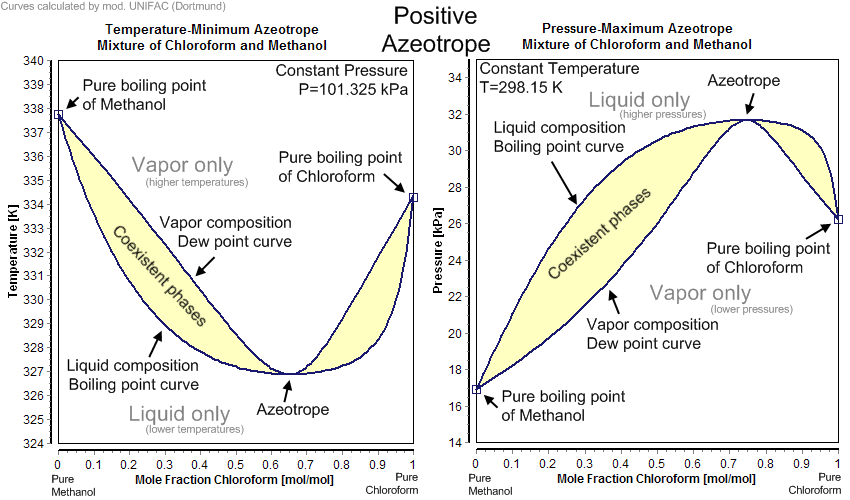
\includegraphics[width=0.48\textwidth, frame]{pos_azeo.png}
    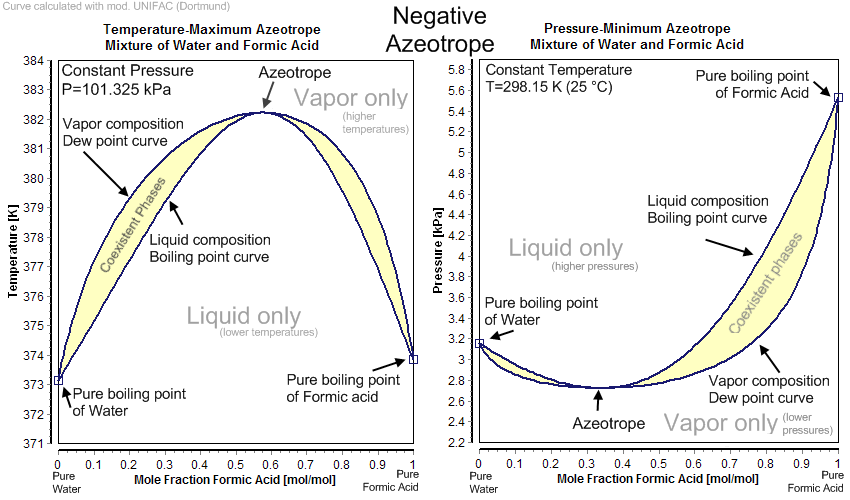
\includegraphics[width=0.48\textwidth, frame]{neg_azeo.png}
\end{figure}
\begin{minipage}[t]{0.55\textwidth}
    \begin{figure}[H]
        \centering
        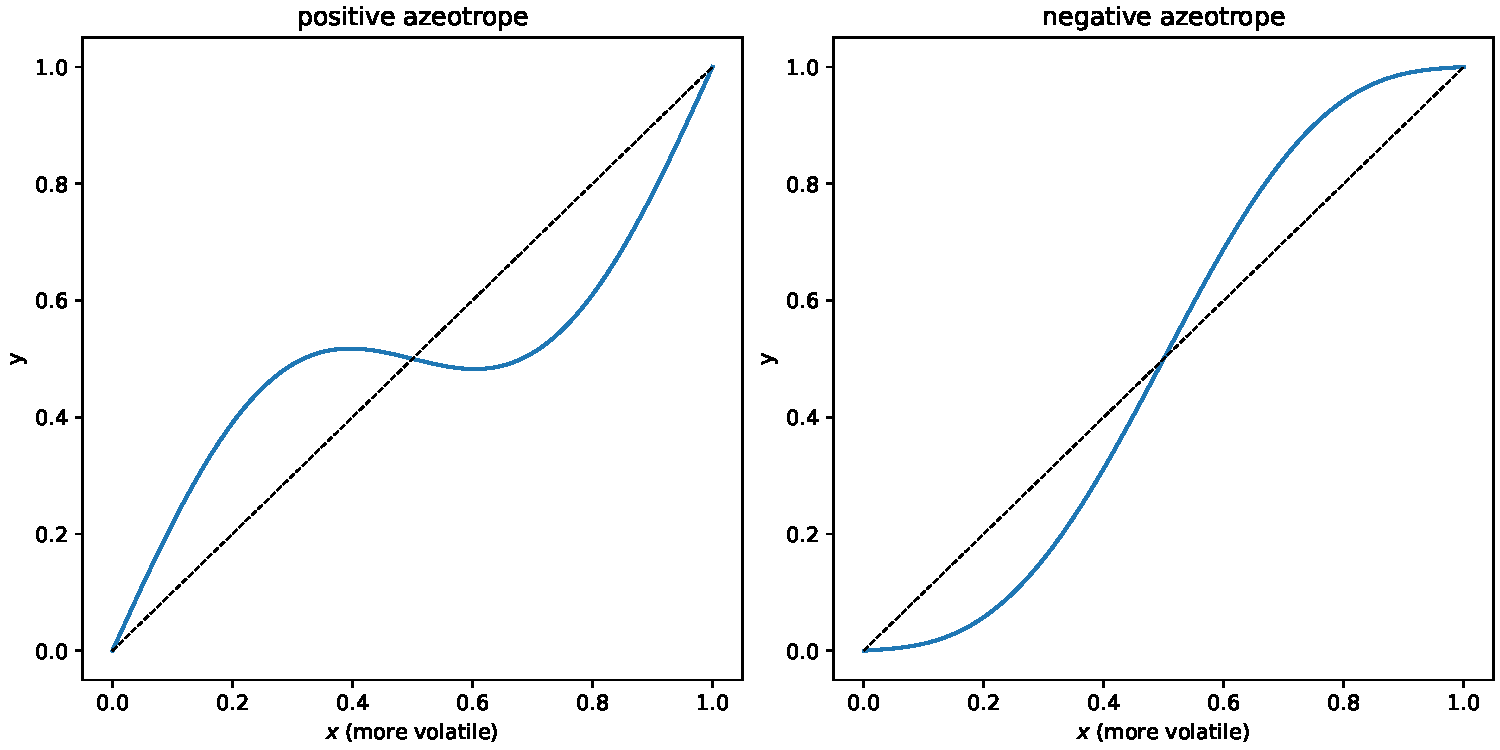
\includegraphics[width=0.99\textwidth]{xy_azeotropes.pdf}
    \end{figure}
\end{minipage}
\begin{minipage}[t]{0.37\textwidth}
    relative volatility
    \[\alpha_{12} = \frac{K_1}{K_2}\]
    \begin{itemize}
        \item relative volatility = 1 at azeotrope
        \item if pure component limits are on opposite sides of 1, an azeotrope likely exists
    \end{itemize}
\end{minipage}


\begin{minipage}[t]{0.3\textwidth}
    reflux ratio, $q$
    \[q = \frac{L}{D}\]
\end{minipage}
\begin{minipage}[t]{0.3\textwidth}
    upper operating line
    \[y = \frac{x_{D}}{1+q} + \frac{x_{i}q}{1+q}\]
    slope less than 1
\end{minipage}
\begin{minipage}[t]{0.3\textwidth}
    lower operating line
    \[y = x \left(\frac{ q+\frac{F}{D}}{q+1} \right) - x_{b} \left( \frac{\frac{F}{D} -1}{q+1} \right)\]
    slope greater than 1
\end{minipage}

\begin{figure}[H]
    \centering
    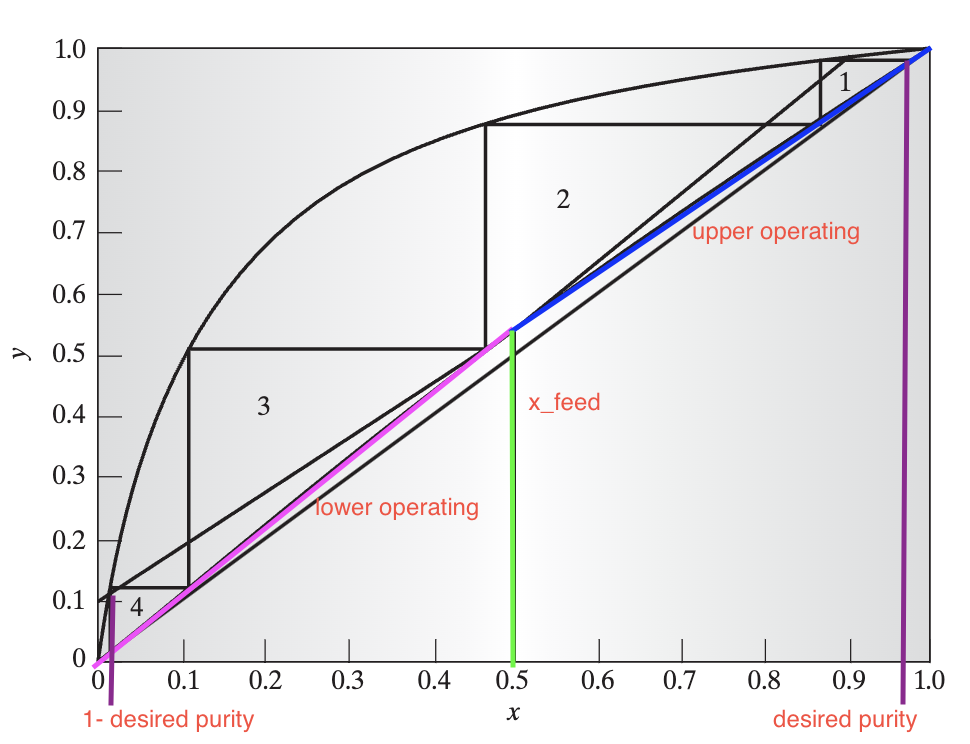
\includegraphics[width=0.5\textwidth]{mct_method.png}
\end{figure}

\begin{minipage}[t]{0.48\textwidth}
    \subsubsection*{activity coeff models}
    one constant margules
    \[ \underline{G}^{\text{ex}} = A x_1 x_2 \hspace{3em} RT \ln \gamma_1 = Ax_2^2 \]
    \begin{itemize}
        \item symmetric!
    \end{itemize}
\end{minipage}
\begin{minipage}[t]{0.48\textwidth}
    Redlich-Kister
    \[ \underline{G}^{\text{ex}} =  x_1 x_2 \left\{ A + B (x_1 - x_2) + C (x_1 - x_2)^2  \dots \right\}  \]
    two constant margules (redlich, but only A,B nonzero)
    \[RT \ln \gamma_1 = \alpha_1 x_2^2 + \beta_1 x_2^3 \]
    \[RT \ln \gamma_2 = \alpha_2 x_1^2 + \beta_2 x_1^3 \]
    \[  \alpha_i = A + 3(-1)^{i+1}B  \]
    \[  \beta_i = 4(-1)^i B \]
    \begin{itemize}
        \item no longer necessarily symmetric
    \end{itemize}
\end{minipage}







\end{document}